\documentclass[tikz,border=10pt]{standalone}
\usepackage{tikz}
\usetikzlibrary{automata, positioning, arrows.meta, bending}
\usetikzlibrary{calc}

\begin{document}

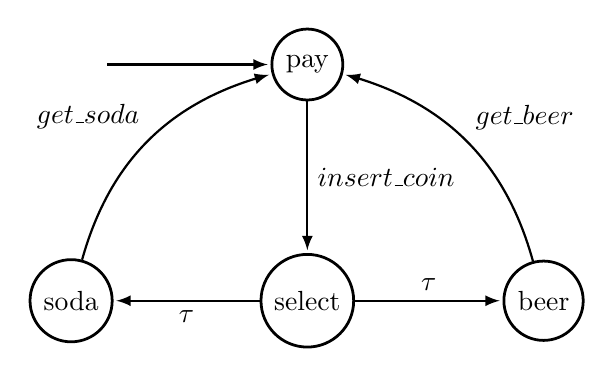
\begin{tikzpicture}[shorten >=1pt,node distance=3cm,on grid,auto,line width=1pt, every edge/.style={draw, -latex, thick}]
   \node[state] (q_2) {pay};
   \node[state,draw=none] (null) [left=of q_2] {};
   \node[state] (q_1) [below =of q_2]  {select};
   \node[state] (q_4) [left=of q_1]{soda};
   \node[state] (q_5) [right=of q_1] {beer};
   

   \path[->]
    (q_4) edge[bend left]  node {$get\_soda$} (q_2)
    (q_5) edge [bend right]  node [above right]{$get\_beer$} (q_2)
    (q_2) edge  node {$insert\_coin$} (q_1)
    (q_1) edge  node {$\tau$} (q_4)
    (q_1) edge node{$\tau$} (q_5)
    (null) edge (q_2);
    
\end{tikzpicture}

\end{document}
